\begin{frame}[fragile]
\frametitle{¿Qué queremos en LA-CoNGA?}
\begin{columns}[c] % The "c" option specifies centered vertical alignment while the "t" option is used for top vertical alignment

\column{.58\textwidth}

\begin{itemize}
	\item {\bf \color{LCredInst} LA-CoNGA physics} desarrolla un programa de {\bf  \color{LCblueInst} especialización en Física avanzada} 
	\item Este programa {\bf  \color{logoyellow} se inserta como especialización en las maestrías de Física} de los socios de LA (8 universidades)
	\item Está inspirado en los {\bf  \color{logobrownD} protocolos de Bolonia (60 ECTS)}
	\item Se basa sobre tres pilares
	\begin{itemize}
		\item Ciencia
		\item Datos
		\item Instrumentación
		\end{itemize}
	\item Se guía por los principios de {\bf  \color{LCblueSec1} ciencia y educación abierta}
\end{itemize}


\column{.38\textwidth} % Right column and width
\begin{center}
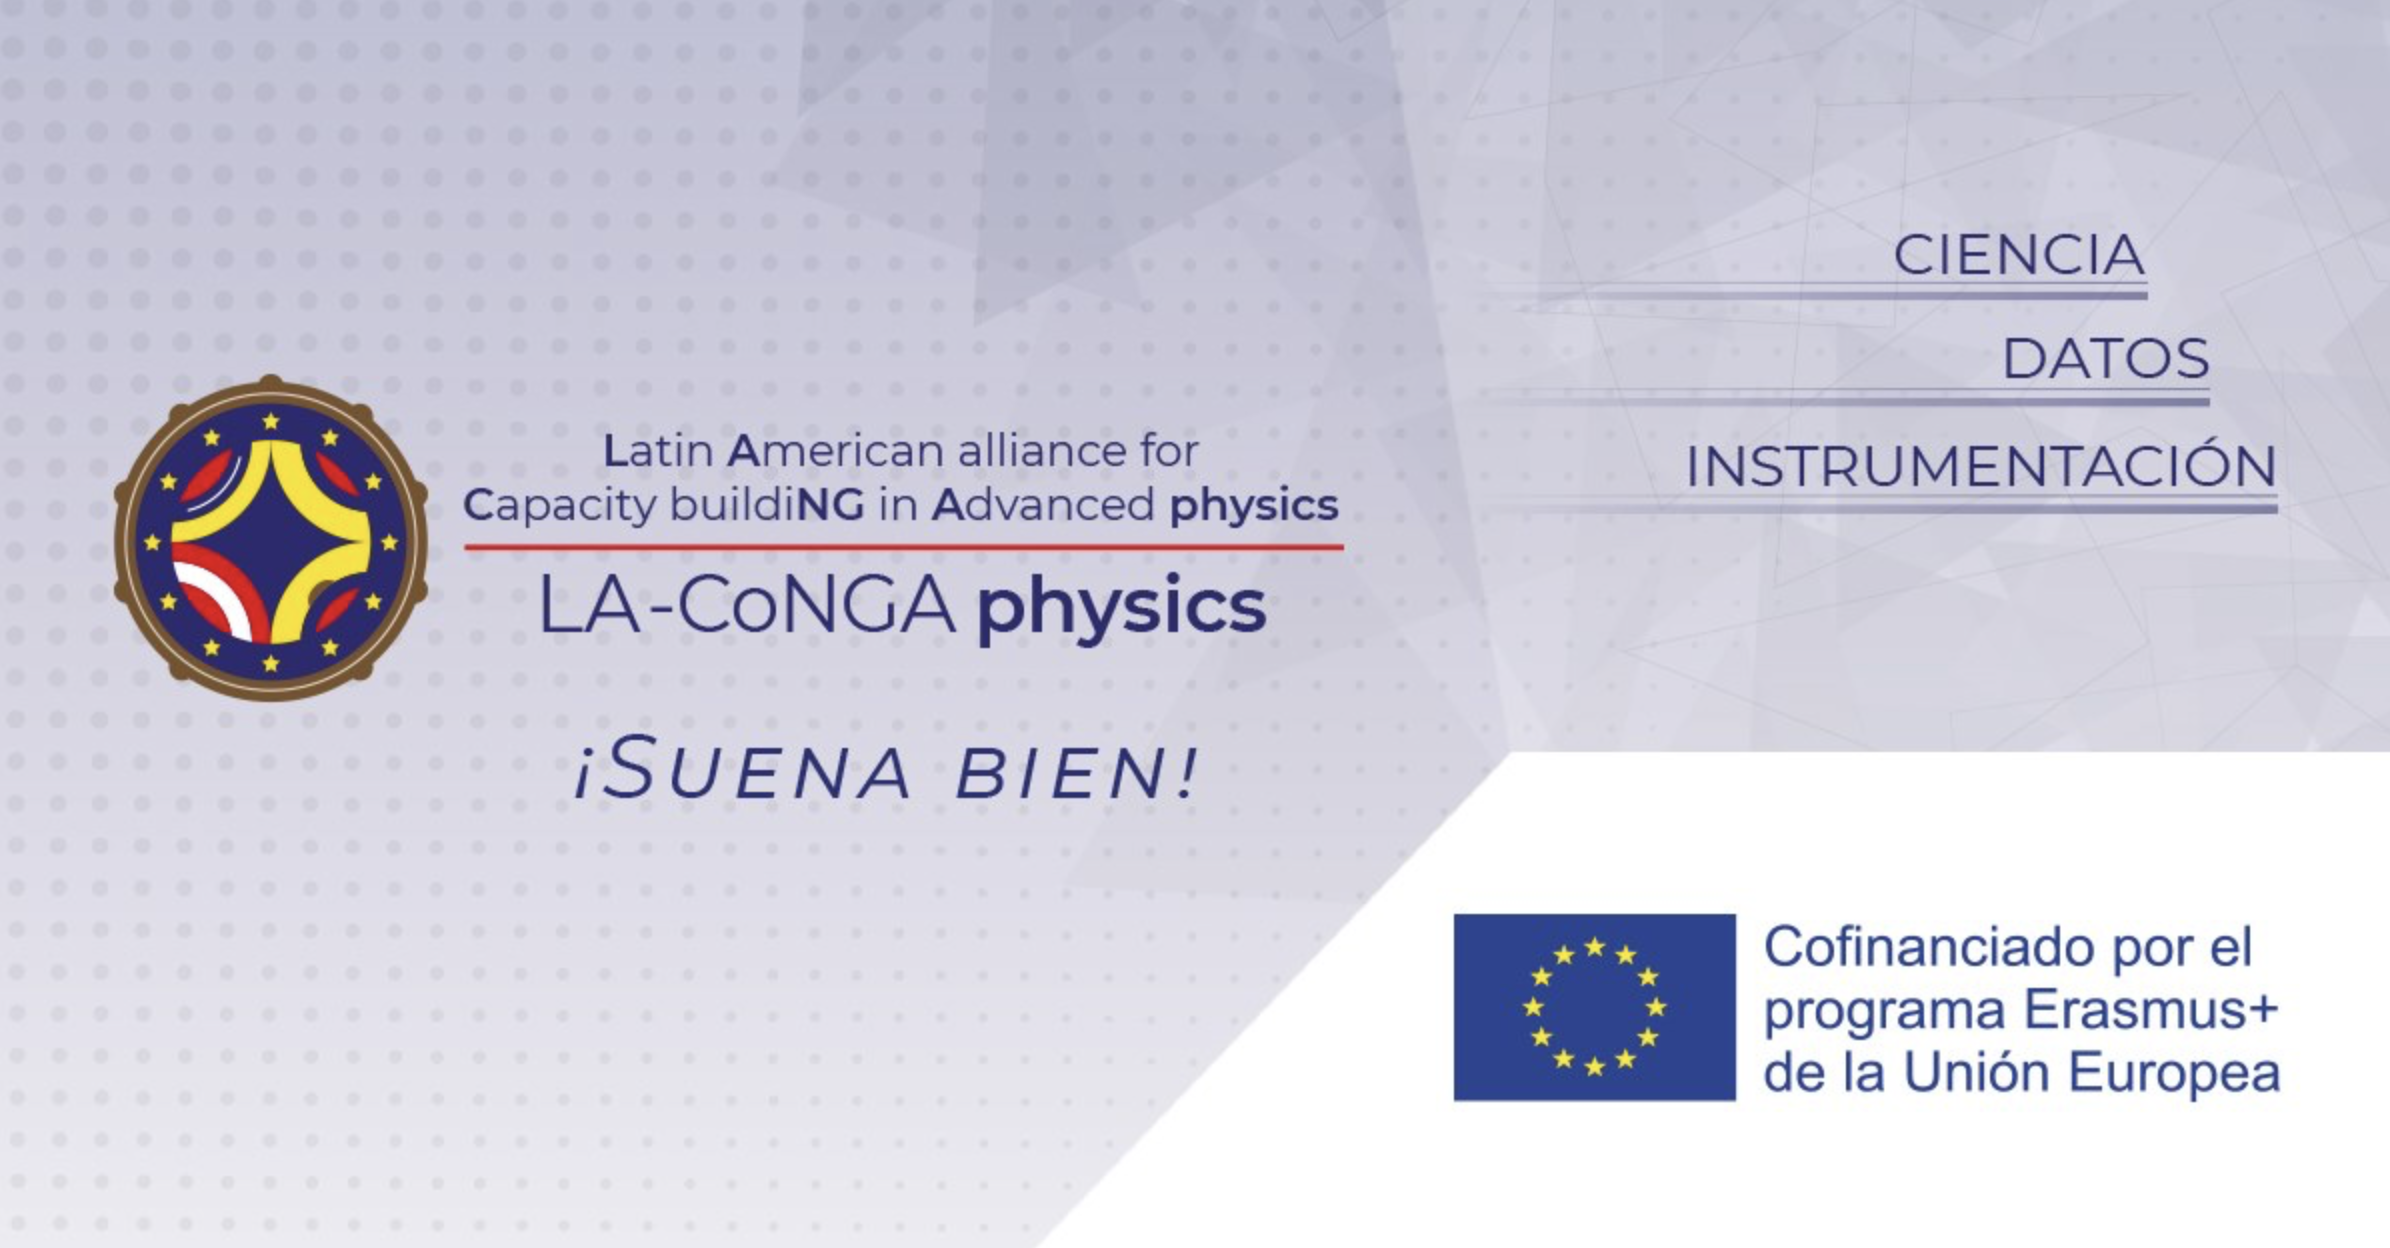
\includegraphics[scale=0.07]{imagenes/principios.png}
\end{center}

\end{columns}


\end{frame}

\begin{frame}[fragile]
\frametitle{LA-CoNGA quiere estudiar Física de Altas Energías}
\begin{center}
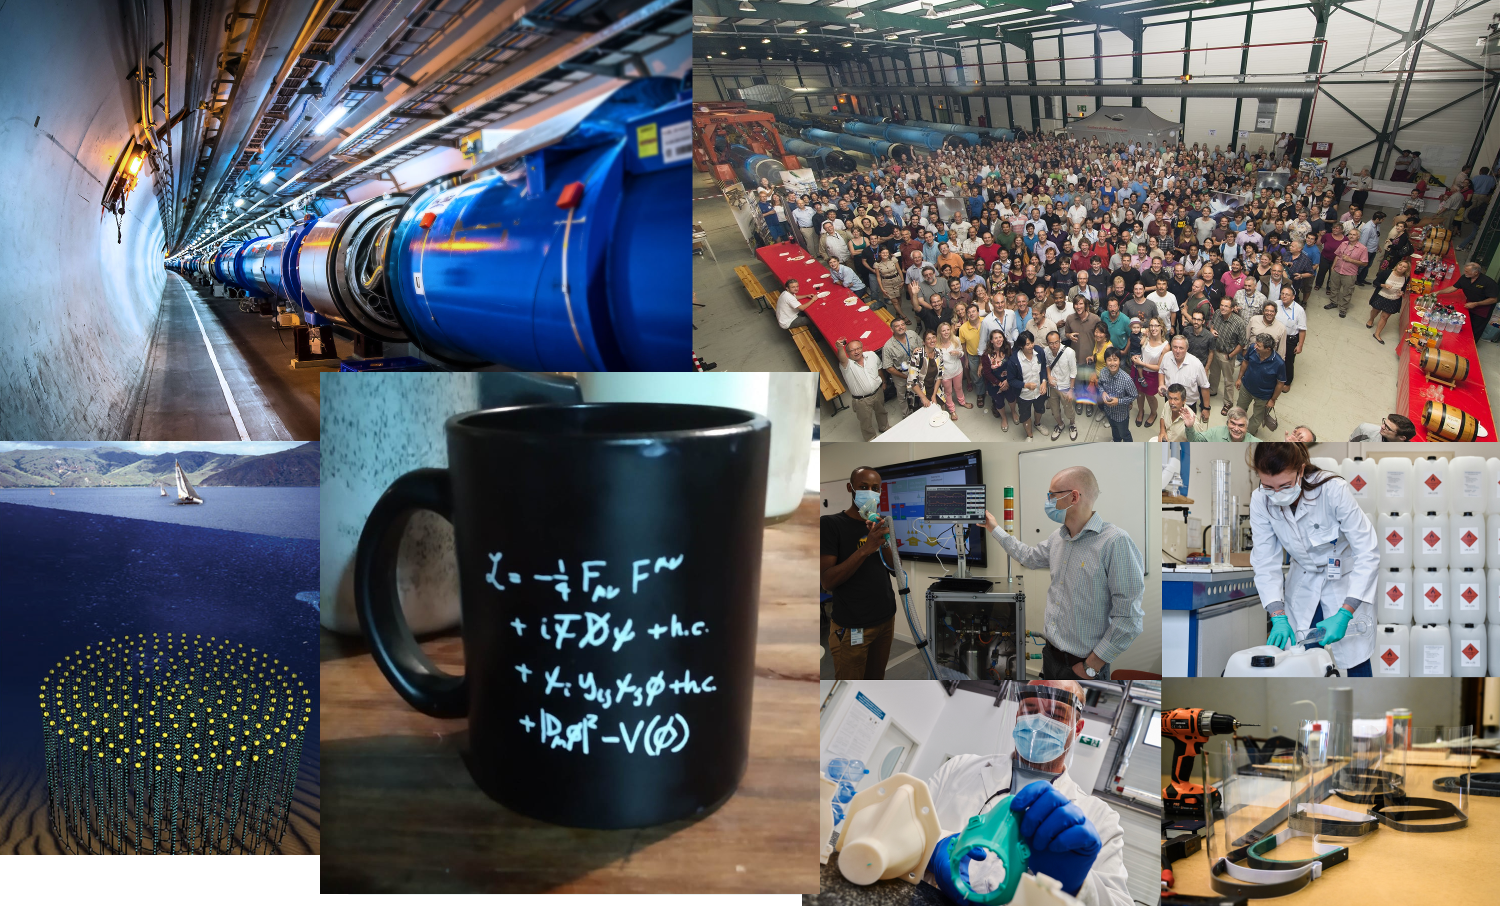
\includegraphics[scale=0.91]{imagenes/fisicaAE.png}
\end{center}
\end{frame}


\begin{frame}[fragile]
\frametitle{LA-CoNGA quiere estudiar Física de los Sistemas Complejos}
\begin{center}
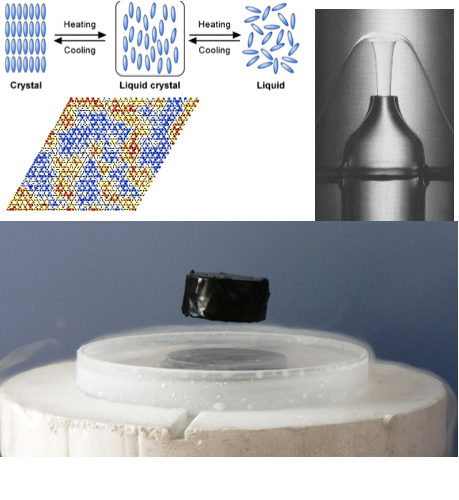
\includegraphics[scale=0.9]{imagenes/fisicaSC1.png}
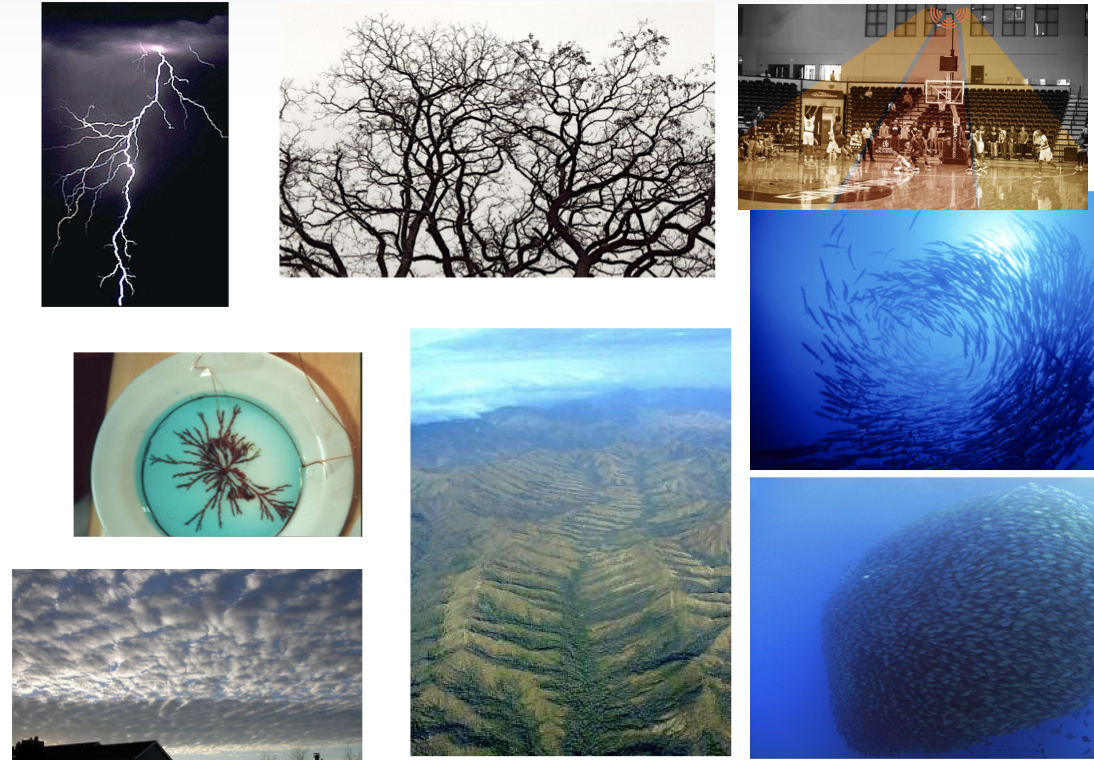
\includegraphics[scale=0.2]{imagenes/fisicaSC2.png}
\end{center}
\end{frame}


